\documentclass[review]{elsarticle}

\usepackage[colorlinks]{hyperref}
\usepackage[colorinlistoftodos]{todonotes}
\usepackage{verbatim}
\usepackage[utf8]{inputenc}
\usepackage[T1]{fontenc}
\usepackage{adjustbox}
\usepackage{multirow}
\usepackage{longtable}
\usepackage{booktabs}
\usepackage{lineno,hyperref}
\usepackage{listings}
\modulolinenumbers[5]

\journal{DAACH}

%%%%%%%%%%%%%%%%%%%%%%%
%% Elsevier bibliography styles
%%%%%%%%%%%%%%%%%%%%%%%
%% To change the style, put a % in front of the second line of the current style and
%% remove the % from the second line of the style you would like to use.
%%%%%%%%%%%%%%%%%%%%%%%

%% Numbered
%\bibliographystyle{model1-num-names}

%% Numbered without titles
%\bibliographystyle{model1a-num-names}

%% Harvard 
%\bibliographystyle{model2-names.bst}\biboptions{authoryear}

%% Vancouver numbered
%\usepackage{numcompress}\bibliographystyle{model3-num-names}

%% Vancouver name/year
%\usepackage{numcompress}\bibliographystyle{model4-names}\biboptions{authoryear}

%% APA style
\bibliographystyle{model5-names}\biboptions{authoryear}

%% AMA style
%\usepackage{numcompress}\bibliographystyle{model6-num-names}

%% `Elsevier LaTeX' style
%\bibliographystyle{elsarticle-num}
%%%%%%%%%%%%%%%%%%%%%%%

\begin{document}

\begin{frontmatter}

%% Title, authors and addresses

\title{Lithic Morphological Organisation: Gahagan Bifaces from the Southern Caddo Area}

%% use the tnoteref command within \title for footnotes;
%% use the tnotetext command for the associated footnote;
%% use the fnref command within \author or \address for footnotes;
%% use the fntext command for the associated footnote;
%% use the corref command within \author for corresponding author footnotes;
%% use the cortext command for the associated footnote;
%% use the ead command for the email address,
%% and the form \ead[url] for the home page:
%%
%% \title{Title\tnoteref{label1}}
%% \tnotetext[label1]{}
%% \author{Name\corref{cor1}\fnref{label2}}
%% \ead{email address}
%% \ead[url]{home page}
%% \fntext[label2]{}
%% \cortext[cor1]{}
%% \address{Address\fnref{label3}}
%% \fntext[label3]{}


%% use optional labels to link authors explicitly to addresses:
%% \author[label1,label2]{<author name>}
%% \address[label1]{<address>}
%% \address[label2]{<address>}
%% Group authors per affiliation:
\author{Robert Z. Selden, Jr.\textsuperscript{a,b,c*}, John E. Dockall\textsuperscript{d,e}, and Harry J. Shafer\textsuperscript{f}}
\address[1]{Heritage Research Center, Stephen F. Austin State University, United States}
\address[2]{Cultural Heritage Department, Jean Monnet University, France}
\address[3]{ORCID ID \href{http://orcid.org/0000-0002-1789-8449}{0000-0002-1789-8449}}
\address[4]{Prewitt and Associates, Inc., United States}
\address[5]{ORCID ID \href{http://orcid.org/0000-0002-0940-7144}{0000-0002-0940-7144}}
\address[6]{Department of Anthropology, Texas A\&M University, United States}
\cortext[cor1]{Corresponding author, Robert Z. Selden, Jr. (zselden@sfasu.edu)}

\begin{abstract}
%% Text of abstract 
This analysis of Gahagan biface morphology enlists the three largest samples of Gahagan bifaces, to include that of the type site (Gahagan Mound) as well as the Mounds Plantation and George C. Davis sites. Results indicate a significant difference in Gahagan biface morphology at the Mounds Plantation site when compared with Gahagan bifaces from the Gahagan Mound and George C. Davis sites. Tests for allometry and asymmetry were not significant. The test of morphological disparity indicates that Gahagan bifaces produced at the Mounds Plantation site occupy a more restricted range of morphospace than those produced at Gahagan Mound, providing indirect evidence for standardisation and diversity in Caddo biface production. While the sample includes a wide range of morphological variability, the test of morphological integration indicates that Gahagan bifaces are significantly integrated, meaning that those traits used to characterise their shape (blade and base) vary in a coordinated manner. These results articulate with a shift in Caddo bottle morphology over the same geography, potentially indicating two previously unrecognised and morphologically-distinct lithic and ceramic production areas.
\end{abstract}

\begin{keyword}
American Southeast \sep Caddo \sep 3D \sep geometric morphometrics \sep morphological integration \sep morphological disparity \sep virtual archaeology
\end{keyword}

\end{frontmatter}

\linenumbers

\section{Gahagan bifaces}

\citet[173-174]{RN800} originally termed the large thin bifaces from tomb contexts at the George C. Davis site to be similar in form, but not technology, to the Copena points discovered in northern Alabama and described by \citet[301-306]{RN11562}. The chronological placement of Gahagan bifaces is Late Prehistoric with a distribution that includes central, east-central, and east Texas with a limited presence in south Texas and Louisiana \citep[230]{RN5629}. Previous mortuary occurrences of Gahagan bifaces have been reported from Gahagan Mound \citep{RN5274} and Mounds Plantation \citep{RN2740} in northwestern Louisiana (Figure ~\ref{fig:SCA}). Clarence H. Webb later suggested Gahagan as a typological term to replace Copena at the 1970 Caddo Conference \citep[229]{RN3682}; however, it was not until 2006 that a morphological and technological description was advanced \citep[22]{RN4924}:

\begin{quote}
Gahagan bases are either slightly concave or straight, and the lateral edges are slightly recurved, contracting slightly below the base and reaching maximum width about mid-length on the less-reduced examples. Lateral edges are finished and retouched by fine pressure flaking. Thinning flakes expand out from the platform and terminate near the middle of the blade rather than carrying across, indicating well-controlled thinning skill. Cross sections are faintly lenticular to almost flat. Retouching reduces the size and curvature of the blade to the extent that the blades may become almost triangular but usually retain the recurved blade form. Bevelling along the lower part of the left edge is a rare, uncharacteristic method of resharpening. The knives may display moderate to extensive use wear in the form of microflake damage or `nicking' and edge abrasion. The overall size depends largely on the degree of retouch.
\end{quote}

\begin{figure}[ht]\centering
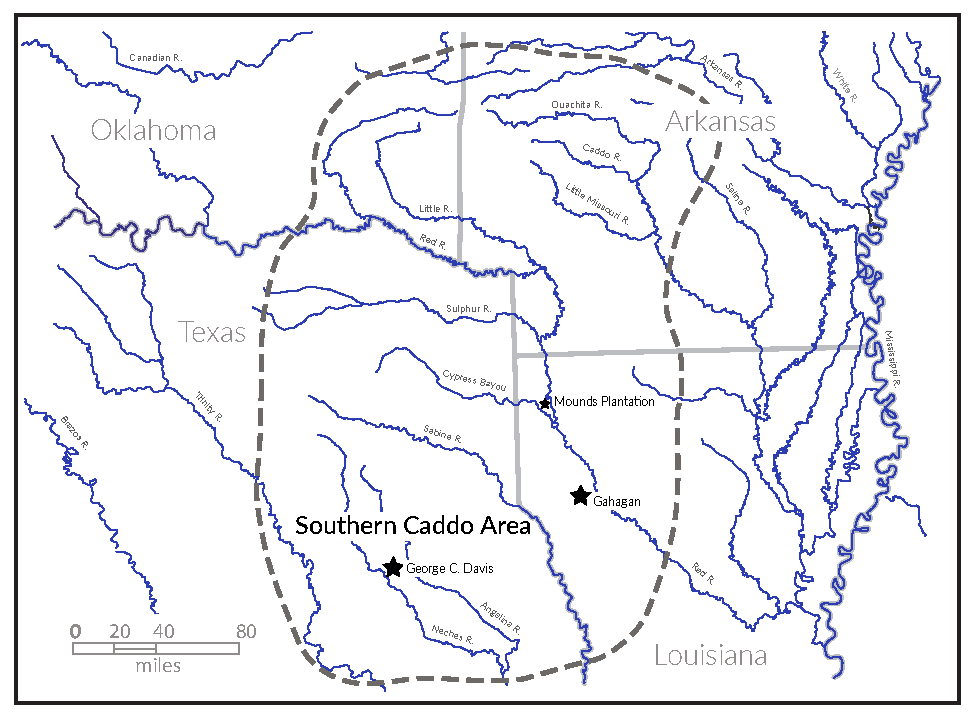
\includegraphics[width=\linewidth]{SCA}
\caption{Location of the Gahagan Mound, Mounds Plantation, and George C. Davis sites in the Southern Caddo Area.}
\label{fig:SCA}
\end{figure}

Researchers initially considered the majority of Gahagan bifaces to be manufactured of Edwards chert but subsequent studies of those bifaces from Davis \citep{RN4924}, Mounds Plantation \citep{RN11561} and other locations \citep{RN1001} have documented a surprising diversity of raw materials in addition to Edwards. Other raw materials represented include chert sources in the Kiamichi Mountains of southeastern Oklahoma, and Woodford, Battiest, Big Fork and Ogallala cherts \citep{RN1001}.

Given the significance of blade and base shape to the definition of the Gahagan type, only intact or reconstructed specimens were used in this analysis (Table ~\ref{tab:Tab1}). While comparisons and reference to these three assemblages of Gahagan bifaces occur in the gray literature \citep{RN11571,RN11565,RN11570,RN11568}, these specimens have not previously been aggregated for a comprehensive morphological analysis. Preliminary observations point to significant morphological differences between Gahagan bifaces recovered from Mounds Plantation and those found at the Gahagan Mound and George C. Davis sites. Given the importance of these bifaces to defining components of Caddo sites that may articulate with Formative or Early Caddo occupations, additional tests for morphological disparity, and morphological integration of the base and blade were used to further expound upon the quiddity of the Gahagan biface type.

\begin{center}
\footnotesize
\begin{longtable}{lccccc}
\caption{\small{Sample of Gahagan bifaces included in the study.}} \label{tab:Tab1} \\

% \hline
\toprule
\multicolumn{1}{l}{Specimen} & \multicolumn{1}{c}{Trinomial} & \multicolumn{1}{c}{Context}& \multicolumn{1}{c}{Site Name} & \multicolumn{1}{c}{Repository}\\ 
% \hline 
\midrule
\endfirsthead

\multicolumn{3}{c}%
{{\tablename\ \thetable{} -- continued from previous page}} \\
% \hline
\midrule
\multicolumn{1}{l}{Specimen} & \multicolumn{1}{c}{Trinomial} & \multicolumn{1}{c}{Context}& \multicolumn{1}{c}{Site Name} & \multicolumn{1}{c}{Repository}\\ 
% \hline 
\midrule
\endhead

% \hline 
\midrule
\multicolumn{4}{r}{{Continued on next page}} \\ 
% \hline
\endfoot

% \hline
\bottomrule
\endlastfoot

		3Ba90 & 16CD12 & Burial Pit 1 & Mounds Plantation & LSEM\\
		3Bb1 & 16CD12 & Burial Pit 2 & Mounds Plantation & LSEM\\
		3Bb3 & 16CD12 & Burial Pit 2 & Mounds Plantation & LSEM\\
		3Bb4 & 16CD12 & Burial Pit 2 & Mounds Plantation & LSEM\\
		3Bb5 & 16CD12 & Burial Pit 2 & Mounds Plantation & LSEM\\
		3Bb6 & 16CD12 & Burial Pit 2 & Mounds Plantation & LSEM\\
		3Bb7 & 16CD12 & Burial Pit 2 & Mounds Plantation & LSEM\\
		3Bb8 & 16CD12 & Burial Pit 5 & Mounds Plantation & LSEM\\
		BlkThn & 16CD12 & Burial Pit 2 & Mounds Plantation & LSEM\\
		Case2LG & 16CD12 & Burial Pit 2 & Mounds Plantation & LSEM\\
		Case2SM & 16CD12 & Burial Pit 5 & Mounds Plantation & LSEM\\
		LGGray & 16CD12 & Burial Pit 8 & Mounds Plantation & LSEM\\
		489 & 16RR1 & Burial Pit 2 & Gahagan Mound & LSEM\\
		490 & 16RR1 & Burial Pit 2 & Gahagan Mound & LSEM\\
		532 & 16RR1 & Burial Pit 2 & Gahagan Mound & LSEM\\
		533 & 16RR1 & Burial Pit 2 & Gahagan Mound & LSEM\\
		541 & 16RR1 & Burial Pit 2 & Gahagan Mound & LSEM\\
		542 & 16RR1 & Burial Pit 2 & Gahagan Mound & LSEM\\
		543 & 16RR1 & Burial Pit 2 & Gahagan Mound & LSEM\\
		544 & 16RR1 & Burial Pit 2 & Gahagan Mound & LSEM\\
		545 & 16RR1 & Burial Pit 2 & Gahagan Mound & LSEM\\
		546 & 16RR1 & Burial Pit 2 & Gahagan Mound & LSEM\\
		547 & 16RR1 & Burial Pit 2 & Gahagan Mound & LSEM\\
		548 & 16RR1 & Burial Pit 2 & Gahagan Mound & LSEM\\
		549 & 16RR1 & Burial Pit 2 & Gahagan Mound & LSEM\\
		550 & 16RR1 & Burial Pit 2 & Gahagan Mound & LSEM\\
		551 & 16RR1 & Burial Pit 2 & Gahagan Mound & WMNSU\\
		569 & 16RR1 & Burial Pit 2 & Gahagan Mound & LSEM\\
		593 & 16RR1 & Burial Pit 3 & Gahagan Mound & LSEM\\
		605 & 16RR1 & Burial Pit 3 & Gahagan Mound & LSEM\\
		606 & 16RR1 & Burial Pit 3 & Gahagan Mound & LSEM\\
		607 & 16RR1 & Burial Pit 3 & Gahagan Mound & LSEM\\
		608 & 16RR1 & Burial Pit 3 & Gahagan Mound & LSEM\\
		609 & 16RR1 & Burial Pit 3 & Gahagan Mound & LSEM\\
		610 & 16RR1 & Burial Pit 3 & Gahagan Mound & LSEM\\
		611 & 16RR1 & Burial Pit 3 & Gahagan Mound & LSEM\\
		612 & 16RR1 & Burial Pit 3 & Gahagan Mound & LSEM\\
		613 & 16RR1 & Burial Pit 3 & Gahagan Mound & LSEM\\
		614 & 16RR1 & Burial Pit 3 & Gahagan Mound & LSEM\\
		622 & 16RR1 & Burial Pit 3 & Gahagan Mound & LSEM\\
		666 & 16RR1 & Burial Pit 3 & Gahagan Mound & LSEM\\
		ET221-993 & 41CE19 & 6L3 & George C. Davis & TARL\\
		ET221-1016 & 41CE19 & F3 & George C. Davis & TARL\\
		ET221-1260A & 41CE19 & 21R14 & George C. Davis & TARL\\
		4078-8 & 41CE19 & F134 & George C. Davis & TARL\\
		4078-9 & 41CE19 & F134 & George C. Davis & TARL\\
		4078-11 & 41CE19 & F134 & George C. Davis & TARL\\
		4078-12 & 41CE19 & F134 & George C. Davis & TARL\\
		4078-13 & 41CE19 & F134 & George C. Davis & TARL\\
		4078-14 & 41CE19 & F134 & George C. Davis & TARL\\
		4078-14B & 41CE19 & F134 & George C. Davis & TARL\\
		4078-22 & 41CE19 & F134 & George C. Davis & TARL\\
		4078-30 & 41CE19 & F134 & George C. Davis & TARL\\
		4078-32 & 41CE19 & F134 & George C. Davis & TARL\\
		4078-45 & 41CE19 & F134 & George C. Davis & TARL\\
		4078-72 & 41CE19 & F134 & George C. Davis & TARL\\
		424-33 & 41CE19 & F119 & George C. Davis & TARL\\
		424-39 & 41CE19 & F119 & George C. Davis & TARL\\
		424-40 & 41CE19 & F119 & George C. Davis & TARL\\
		424-41 & 41CE19 & F119 & George C. Davis & TARL\\
		424-50 & 41CE19 & F119 & George C. Davis & TARL\\
		424-53 & 41CE19 & F119 & George C. Davis & TARL\\
		424-133 & 41CE19 & F119 & George C. Davis & TARL\\
		424-169 & 41CE19 & F119 & George C. Davis & TARL\\
		424-218 & 41CE19 & F119 & George C. Davis & TARL\\
		424-221 & 41CE19 & F119 & George C. Davis & TARL\\
		424-230 & 41CE19 & F119 & George C. Davis & TARL\\
		463-1 & 41CE19 & F119 & George C. Davis & TARL\\
		463-16 & 41CE19 & F119 & George C. Davis & TARL\\
		463-23 & 41CE19 & F119 & George C. Davis & TARL\\
%       \hline
\end{longtable}
\textit{LSEM, Louisiana State Exhibit Museum; WMNSU, Williamson Museum at Northwestern State University; TARL, Texas Archeological Research Laboratory.}
\end{center}

\section{Geometric morphometric analyses of stone tools}

Analyses of lithic shape are neither new or novel, and it is not surprising that geometric morphometrics (GM) (sensu \citet{RN11559}) has captivated analysts of material culture due to the substantive contribution of morphology to lithic typologies \citep{RN11529,RN11528,RN11534}. The first application of GM to archaeologically-recovered artefacts was an analysis of irregular shapes by elliptic Fourier analysis (EFA) \citep{RN4379}, and the adoption of the method by the archaeological community has continued.

EFA has been increasingly employed in lithic analyses, where analysts continue are developing novel approaches that advance archaeological applications \citep{RN11556,RN11529,RN4350,RN4373,RN4338,RN4353,RN11521,RN4143,RN253,RN11534}. Numerous creative research designs have also been presented that address some of the very real challenges associated with the oft-fractured and incomplete specimens abundant in the archaeological record \citep{RN11575,RN11574,RN11539,RN11533}. This approach is particularly useful in instances where homologous landmarks cannot be readily identified; for instance, in cases where both lanceolate and stemmed projectile points are employed in the same analysis.

Landmark-based approaches, like the one applied here, articulate with the rise of the Procrustes paradigm \citep[8]{RN1743}, which have proven utility in archaeological application. This includes a 2D study of blade shape differences in Paleoindian projectile point types where a novel approach to investigating allometry was applied through the use of median point area and size grades to compare shape and size distributions, demonstrating that it is possible to discriminate between some types based upon blade shape "independent of allometry, raw material quality, and resharpening effects" \citep[357]{RN1754}, thus representing a rejection of the reduction thesis \citep{RN11866}. \citet{RN4338x} demonstrated that while reduction is important, it has a greater effect on shape than on size; an observation that is more apparent on blades than on bases, concluding that the two point types used in their study could be successfully segregated despite reduction. Similarly, \citet{RN11528} analysed three Paleoindian projectile points from Florida and found that the types used in his study did not represent continuous variation; rather, they are representative of three discrete groups. 

Like those studies mentioned above, this analysis enlists a landmark-based approach aimed at capitalising upon the variability that occurs along a single plane (widest biface edge); however, 3D data were required to consistently identify the widest edge. Procrustes ANOVAs were used to test whether the intra-type morphology of Gahagan bifaces varies by size and site, a test of morphological disparity to determine relative standardisation and diversity in the sample, and a test of morphological integration to determine whether biface blade and base shapes covary. Additionally, a variety of landmark and semilandmark configurations are in development that will allow for a more robust analysis of 3D morphology associated with specific elements of Gahagan biface morphology.

\section{Methods}

Each of the Gahagan bifaces was scanned with a Creaform GoSCAN 20 at a 0.3 mm resolution in VXelements. Scanner calibration was optimised prior to each scan with positioning targets required for increased accuracy and shutter speed reconfigured in each instance. A clipping plane was established to reduce the amount of superfluous data collected. Following data collection, the resolution of each mesh was increased to 0.1 mm, and the point cloud was transferred to VXmodel where the mesh was rendered following application of the \textit{clean mesh} function, used to remove isolated patches, self-intersections, spikes, small holes, singular vertices, creased edges, narrow triangles, outcropping triangles, narrow bridges, and non-manifold triangles prior to decimation and export as ASCII stl and ASCII ply. The stl functions as a 3D print-ready backup of the scan data, and the ply file was subsequently imported to Geomagic Design X (Dx).

There is a residue adhering to seven of the Gahagan bifaces from the George C. Davis site (Figure ~\ref{fig:FigResidue}) that occurs at variable thicknesses. \citet[228]{RN3682} posits that this residue potentially represents the remains of a sheath. While an interesting aside, the residue does pose a problem for an analysis of 3D geometry. The initial research design (3D) was thus revisited, leading to a reconfiguration of the analysis as a 2D geometric morphometric study that enlisted a landmark configuration similar to that used by \citet[Figure 2]{RN1754}, \citet[Figure 2]{RN1736}, and \citet[Figure 1]{RN11731}. The residue does not occur on all of the George C. Davis specimens, and none of the Gahagan bifaces from the Mounds Plantation or Gahagan Mound sites include a similar residue on their surfaces, making it possible to compare a greater range of surface morphology between those samples. While beyond the scope of this present study, that is an avenue of inquiry worth pursuing should differences in Gahagan biface shape be found to differ among the three sites.

\begin{figure}[ht]\centering
\includegraphics[width=\linewidth]{residue}
\caption{Residue adhering to Gahagan bifaces from Feature 134 at the George C. Davis site; a, 4078-8; b, 4078-9; c, 4078-11; d, 4078-13; e, 4078-72; f, 4078-14B; and g, 4078-14.}
\label{fig:FigResidue}
\end{figure}

\subsection{Alignment and reference geometry}

Following transfer to Dx, each mesh was subjected to a second quality check to eliminate non-manifold poly-vertices, folded poly-faces, dangling poly-faces, small clusters, small poly-faces, non-manifold poly-faces, crossing poly-faces, and small tunnels. The principal assumption in constructing the reference geometry is a reference vector. A sampling ratio of 100 percent was used to extract the reference vector, after which a reference point was added by projecting it atop the mesh surface at the location where the reference vector exits the base of the biface. Each element of reference geometry (vector and point) was then used in an interactive 3-2-1 alignment where the biface was aligned to a global origin, then to the extremes of the lateral edges. 

The widest profile was defined as the location on the mesh that lies furthest from the point at which the reference vector exits the base. To identify that point, a mesh sketch was generated using the planar method---employing the plane located at the base of the biface as the base plane---to sketch a circle around the biface from the top view where the whole of the biface profile was included in the circumference. A 3D surface (cylinder) was extruded around the biface, and the \textit{accuracy analyzer} was used to identify the point on the biface with the lowest deviation from the extruded surface. A plane (MPlane) was then inserted coplanar to the vector and oriented to the widest point, thus bisecting the biface at the location of the widest profile.

Using the MPlane as the basis for a third sketch, a spline was populated along the entirety of the silhouetted profile, and split at the location of each landmark (Table ~\ref{tab:Tbl1}). Four splits were added that include the tip, juncture of the blade/base (widest profile), centre base, and opposing blade/base. Those landmark locations identified at the two points of highest curvature enlist the \textit{curvature} function in Dx, and do not represent arbitrary locations. 

\begin{table}[tbh]\centering
\footnotesize
\caption{Landmarks used in the analysis.}
\centering
\begin{tabular}{lcp{7.5cm}}
\toprule
Landmark & Location & Definition\\
\midrule
Point01 & Tip & Horizontal tangent\\
Point20 & Blade/Base & Point of highest curvature on widest side of biface\\
Point24 & CentreBase & Intersection of vector and external surface of the 3D mesh\\
Point28 & Blade/Base & Point of highest curvature\\
\bottomrule
\end{tabular}
\label{tab:Tbl1}
\end{table}

Two specimens in the George C. Davis sample (4078-8 and 4078-72), both from Feature 134, are missing small sections of their lateral edges (Figure ~\ref{fig:FigResidue}a, e). For the purpose of the GM analysis, these two areas were modelled, where the spline was cut behind the area of highest curvature above and below the missing piece, and a line was inserted to connect the lateral edge above and below the missing piece. This ensures that the spline provides a model that is closer to the (assumed) original intent of the maker. 

Due to the paucity of homologous landmarks or points of morphological correspondence on stone artefacts \citep[81]{RN1730}, reference geometry was constructed around each specimen in a manner that yields a replicable configuration of three landmarks, and 43 equidistant semilandmarks. Landmarks and semilandmarks were populated along the spline, always beginning on the side of the biface determined to include the widest point. Divisions between each section articulate with those of the spline splits, where landmarks were placed at each of the points in Table ~\ref{tab:Tbl1}, with a series of equidistant semilandmarks between (18 for each blade section, and three between each of the basal landmarks; Figure ~\ref{fig:Fig1a}). This constellation of landmarks and semilandmarks allows for tests of morphological integration between the blade and base as well as a test of directional asymmetry \citep{RN4775,RN11619,RN11621,RN11620}.

\begin{figure}[ht]\centering
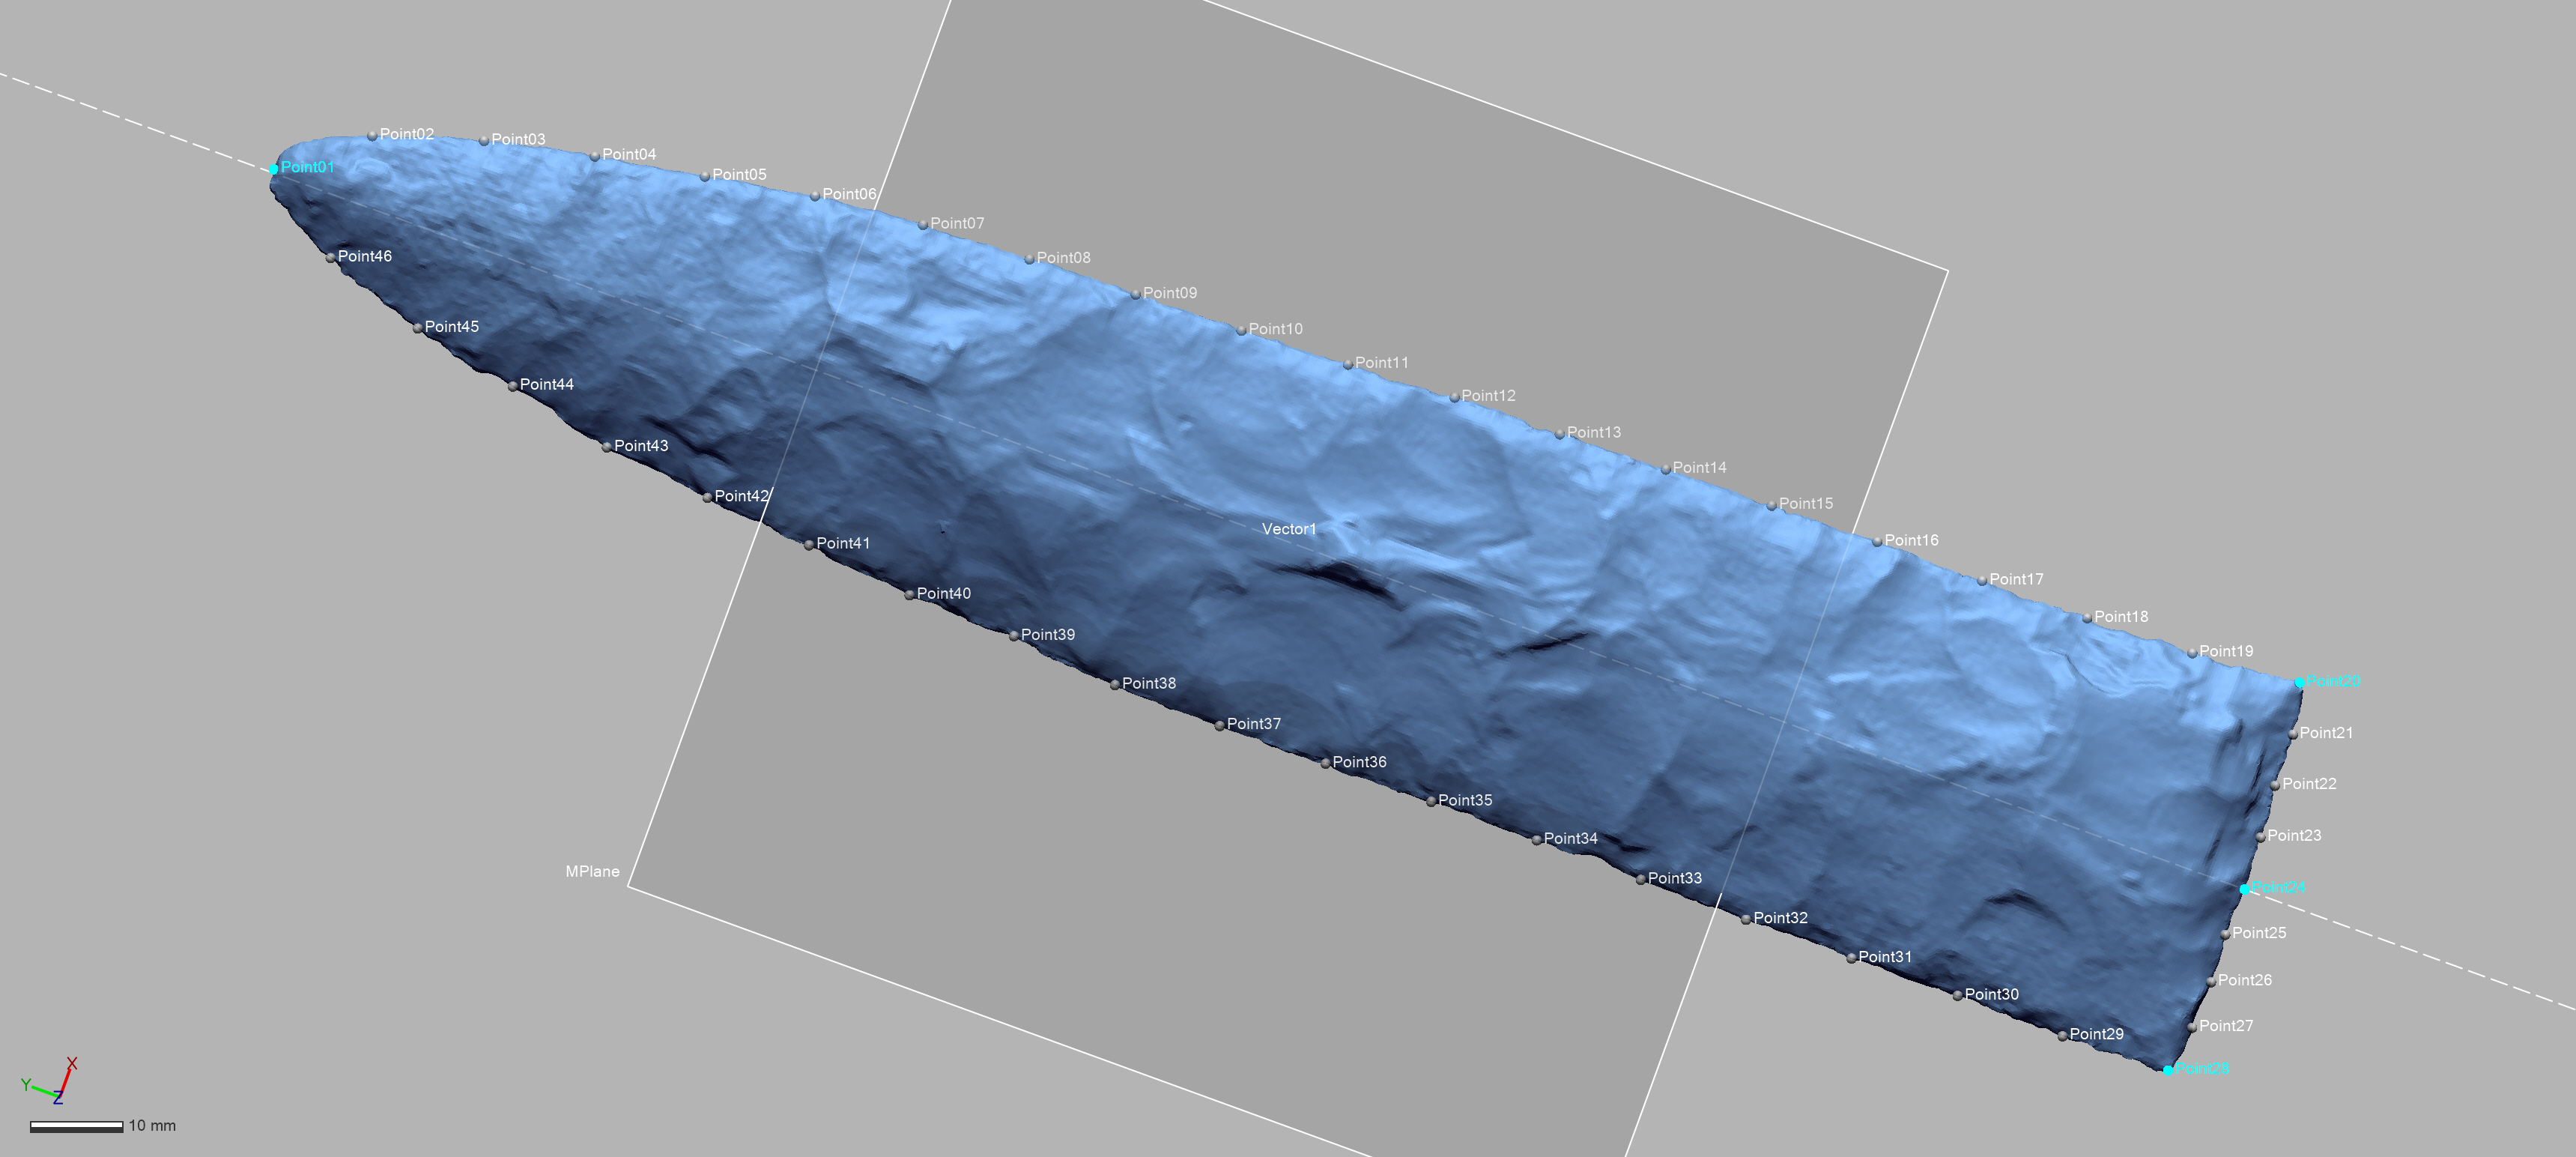
\includegraphics[width=\linewidth]{Fig1a}
\caption{Landmark (blue) and semilandmark (white) placement.}
\label{fig:Fig1a}
\end{figure}

\subsection{Analysis}

Landmarks and equidistant semilandmarks were exported as x, y, and z coordinate data from Dx. Those data were aligned to a global coordinate system \citep{RN11622,RN11623,RN11563}, achieved through generalised Procrustes superimposition \citep{RN478} performed in R 3.4.4 \citep{R} using the \textit{geomorph} library v.3.0.5 \citep{RN11530,RN1774}. Procrustes superimposition translates, scales, and rotates the coordinate data to allow for comparisons among objects \citep{RN11564,RN478}. The \textit{geomorph} package uses a partial Procrustes superimposition that projects the aligned specimens into tangent space subsequent to alignment in preparation for the use of multivariate methods that assume linear space \citep{RN1646,RN11563}.

Principal components analysis \citep{RN1746} was used to visualise shape variation among the bifaces. The shape changes described by each principal axis are commonly visualised using thin-plate spline warping of a reference 3D mesh \citep{RN1731,RN479}. A residual randomisation permutation procedure (RRPP; n=1000 permutations) was used for all Procrustes ANOVAs \citep{RN1655}, which has higher statistical power and a greater ability to identify patterns in the data should they be present \citep{RN1719}. To assess whether shape changes with size (allometry), and differs by group (types and sites), Procrustes ANOVAs \citep{RN1749} were also run that enlist effect-sizes (z-scores) computed as standard deviates of the generated sampling distributions \citep{RN1756}. 

A Procrustes ANOVA and pairwise test was used to identify sites where biface shapes differ. The pairwise test is conceptually similar to trajectory analysis \citep{RN11573,RN1648,RN1776,RN1739} in that pairwise statistics are vector lengths between vectors, but differs since a factorial model is not explicitly needed to contrast vectors between point factor levels nested within group factor levels \citep{RN11530}. Procrustes variance was used to discriminate between groups and compare the amount of shape variation (morphological disparity) across sites \citep{RN11560}, which  is estimated as the Procrustes variance using residuals of linear model fit \citep{RN11530}. 

Morphological integration was tested using a two-block partial least-squares (2B-PLS) analysis to evaluate relationships for two (or more) blocks of variables collected from the same specimens \citep{RN11615,RN11613,RN11614}. Using shape coordinates in all blocks of variables, 2B-PLS can be used to assess morphological integration \citep{RN11616,RN11615,RN11617}. This analysis includes blade shape (Block 1) and base shape (Block 2), allowing for a test of morphological integration between the blocks.

\section{Results}

The mean consensus configuration and Procrustes residuals were calculated for each site by means of a generalised Procrustes analysis (GPA) \citep[Figure 3]{RN1720} (Figure ~\ref{fig:FigGPA}). This initial view of the dataset demonstrates the degree of variation that occurs at each site and in the combined sample. As an exploratory measure, GM methods---to include GPA---aid in clarifying shape differences associated with each population and in the production of novel \textit{a posteriori} hypotheses \citep{RN1720}.  

\begin{figure}[ht]\centering
\includegraphics[width=\linewidth]{gahagan-nwla-gpa-all--ABCD-sm}
\caption{Mean consensus configuration (black) with Procrustes residuals (gray) superimposed by generalised Procrustes analysis for a, Mounds Plantation; b, Gahagan Mound; c, George C. Davis; and d, all specimens.}
\label{fig:FigGPA}
\end{figure}

The mean consensus configuration for the sample from each site points toward a potentially significant difference in Gahagan biface morphology at the Mounds Plantation site. It may also be the case that the Gahagan bifaces produced at Mounds Plantation occupy a smaller range of morphospace than those recovered at Gahagan Mound and George C. Davis. While the mean consensus configurations for Gahagan bifaces from Gahagan Mound and George C. Davis do appear to be similar, there are some notable differences. The bifaces from Gahagan Mound generally include less recurve in the blade, and a base that is more convex than that of the bifaces from George C. Davis, where the mean consensus configuration of the base is slightly concave.

Principal components analysis (PCA) was conducted on scaled, translated, and rotated landmarks, and demonstrates that the first two PCs account for 76 (PC1) and nine (PC2) percent of the variation in Gahagan biface shape (Table ~\ref{tab:Tbl2} and Figure ~\ref{fig:FigPCA}). Together, PC1 and PC2 account for over 86 percent of shape variation for Gahagan bifaces, with each remaining PC representing less than five percent of the variation (Table ~\ref{tab:Tbl2}). The first two PCs are plotted in Figure ~\ref{fig:FigPCA}, where warp grids represent the shape changes along PC1 and PC2. This plot indicates that shape changes associated with PC1 articulate most readily with blades that range from broader at the minimum to narrow at the maximum, and base shapes that range from more concave at the minimum toflat or slightly convex at the maximum. Those shape changes associated with PC2 are dominated by differences in base shapes that range from narrow at minimum to broad at maximum, and blade shapes that are broader at minimum to narrower at maximum.

\begin{table}[tbh]\centering
\footnotesize
\caption{Results of principal components analysis for first 10 PCs (> 98 percent of total variance explained).}
\centering
\begin{tabular}{lp{2cm}p{2cm}p{2cm}}
\toprule
 & SD & PVE & CVE\\
\midrule
PC1 & 0.05939 & 0.76305 & 0.76305\\
PC2 & 0.02132 & 0.09829 & 0.86135\\
PC3 & 0.01504 & 0.04891 & 0.91026\\
PC4 & 0.01041 & 0.02347 & 0.93373\\
PC5 & 0.009359 & 0.018950 & 0.952680\\
PC6 & 0.007708 & 0.012850 & 0.965540\\
PC7 & 0.007231 & 0.011310 & 0.976850\\
PC8 & 0.004334 & 0.004060 & 0.980910\\
PC9 & 0.003663 & 0.002900 & 0.983810\\
PC10 & 0.003434 & 0.002550 & 0.986370\\
\bottomrule
\end{tabular}
\bigskip
\\\textit{SD - standard deviation; PVE - percentage variance explained; CVE - cumulative variance explained.}
\label{tab:Tbl2}
\end{table}

\begin{figure}[ht]\centering
\includegraphics[width=\linewidth]{pca}
\caption{Principal components analysis plot (PC1/PC2) for Gahagan bifaces by site; green, Mounds Plantation; black, Gahagan Mound; red, George C. Davis.}
\label{fig:FigPCA}
\end{figure}

A Procrustes ANOVA was then used to test whether there was a significant difference in biface shape by site. Results of the ANOVA indicate a significant difference in biface shape by site (RRPP = 1000; Rsq = 0.33044; Pr(>F) = 0.001), and a pairwise test of shapes between groups designated by site confirms a significant difference in Gahagan biface shape at the Mounds Plantation site when compared with Gahagan Mound and George C. Davis (Table ~\ref{tab:Tbl3x}).

\begin{table}[tbh]\centering
\footnotesize
\caption{P-values, effect sizes, and least-squares mean distance matrix for advanced Procrustes ANOVA and pairwise test (RRPP = 1000) of Gahagan biface shape.}
\centering
\begin{tabular}{lrrr}
\toprule
 & Gahagan Mound & George C Davis & Mounds Plantation\\
\midrule
Gahagan Mound & 1.000 &  & \\
 & \textit{0.0000000} &  & \\
 & (0.00000000) &  & \\
George C Davis & 0.343 & 1.000 & \\
 & \textit{0.1620967} & \textit{0.0000000} & \\
 & (0.01783345) & (0.00000000) & \\
Mounds Plantation & \textbf{0.001} & \textbf{0.001} & 1.000\\
 & \textit{6.3816976} & \textit{7.8954687} & \textit{0.000000}\\
 & (0.09244913) & (0.10820597) & (0.00000000)\\
\bottomrule
\end{tabular}
\bigskip\\
\textit{Significant differences in bold; effect sizes (z) in italics; least-squares means distance matrix in parentheses.}
\label{tab:Tbl3x}
\end{table}

The test of morphological disparity indicates that while bifaces at both Gahagan Mound and George C. Davis display a greater range of shape variation among individuals relative to other groups, the Gahagan bifaces from Gahagan Mound occupy a significantly greater range of morphospace than those from Mounds Plantation (Table ~\ref{tab:Tbl4x}). This indicates that those bifaces at the Gahagan Mound site encompass a greater range of morphological variability than those produced at the Mounds Plantation site, meaning that Caddo makers at the Mounds Plantation site were participating in a more morphologically-restricted method of biface manufacture.

\begin{table}[htbp]\centering
\footnotesize
\caption{P-values and pairwise absolute differences between variances for the test of morphological disparity (RRPP = 1000).}
\centering
\begin{tabular}{lrrr}
\toprule
 & Gahagan Mound & George C Davis & Mounds Plantation\\
\midrule
Gahagan Mound & 1.000 &  &\\
 & \textit{0.0000000000} &  & \\
George C Davis & 0.640 & 1.000 & \\
 & \textit{0.0007943556} & \textit{0.0000000000} & \\
Mounds Plantation & \textbf{0.039} & 0.089 & 1.000\\
 & \textit{0.0041492880} & \textit{0.0033549324} & \textit{0.000000000}\\
\bottomrule
\end{tabular}
\bigskip\\
\textit{Significant differences in bold; pairwise absolute differences between variances in italics.}
\label{tab:Tbl4x}
\end{table}

A two-block partial least-squares (2B-PLS) analysis was used to test for morphological integration between base and blade shape of the Gahagan biface sample. The results indicate significant morphological integration (1000 random permutations; r-PLS = 0.805; P-value = 0.001), indicating that blade shape and base shape vary in a coordinated manner (Figure ~\ref{fig:FigMorphInteg}). In general terms, longer and thinner bifaces were found to articulate with a slightly convex base, while shorter and broader bifaces articulate with a slightly concave base.

\begin{figure}[htbp]\centering
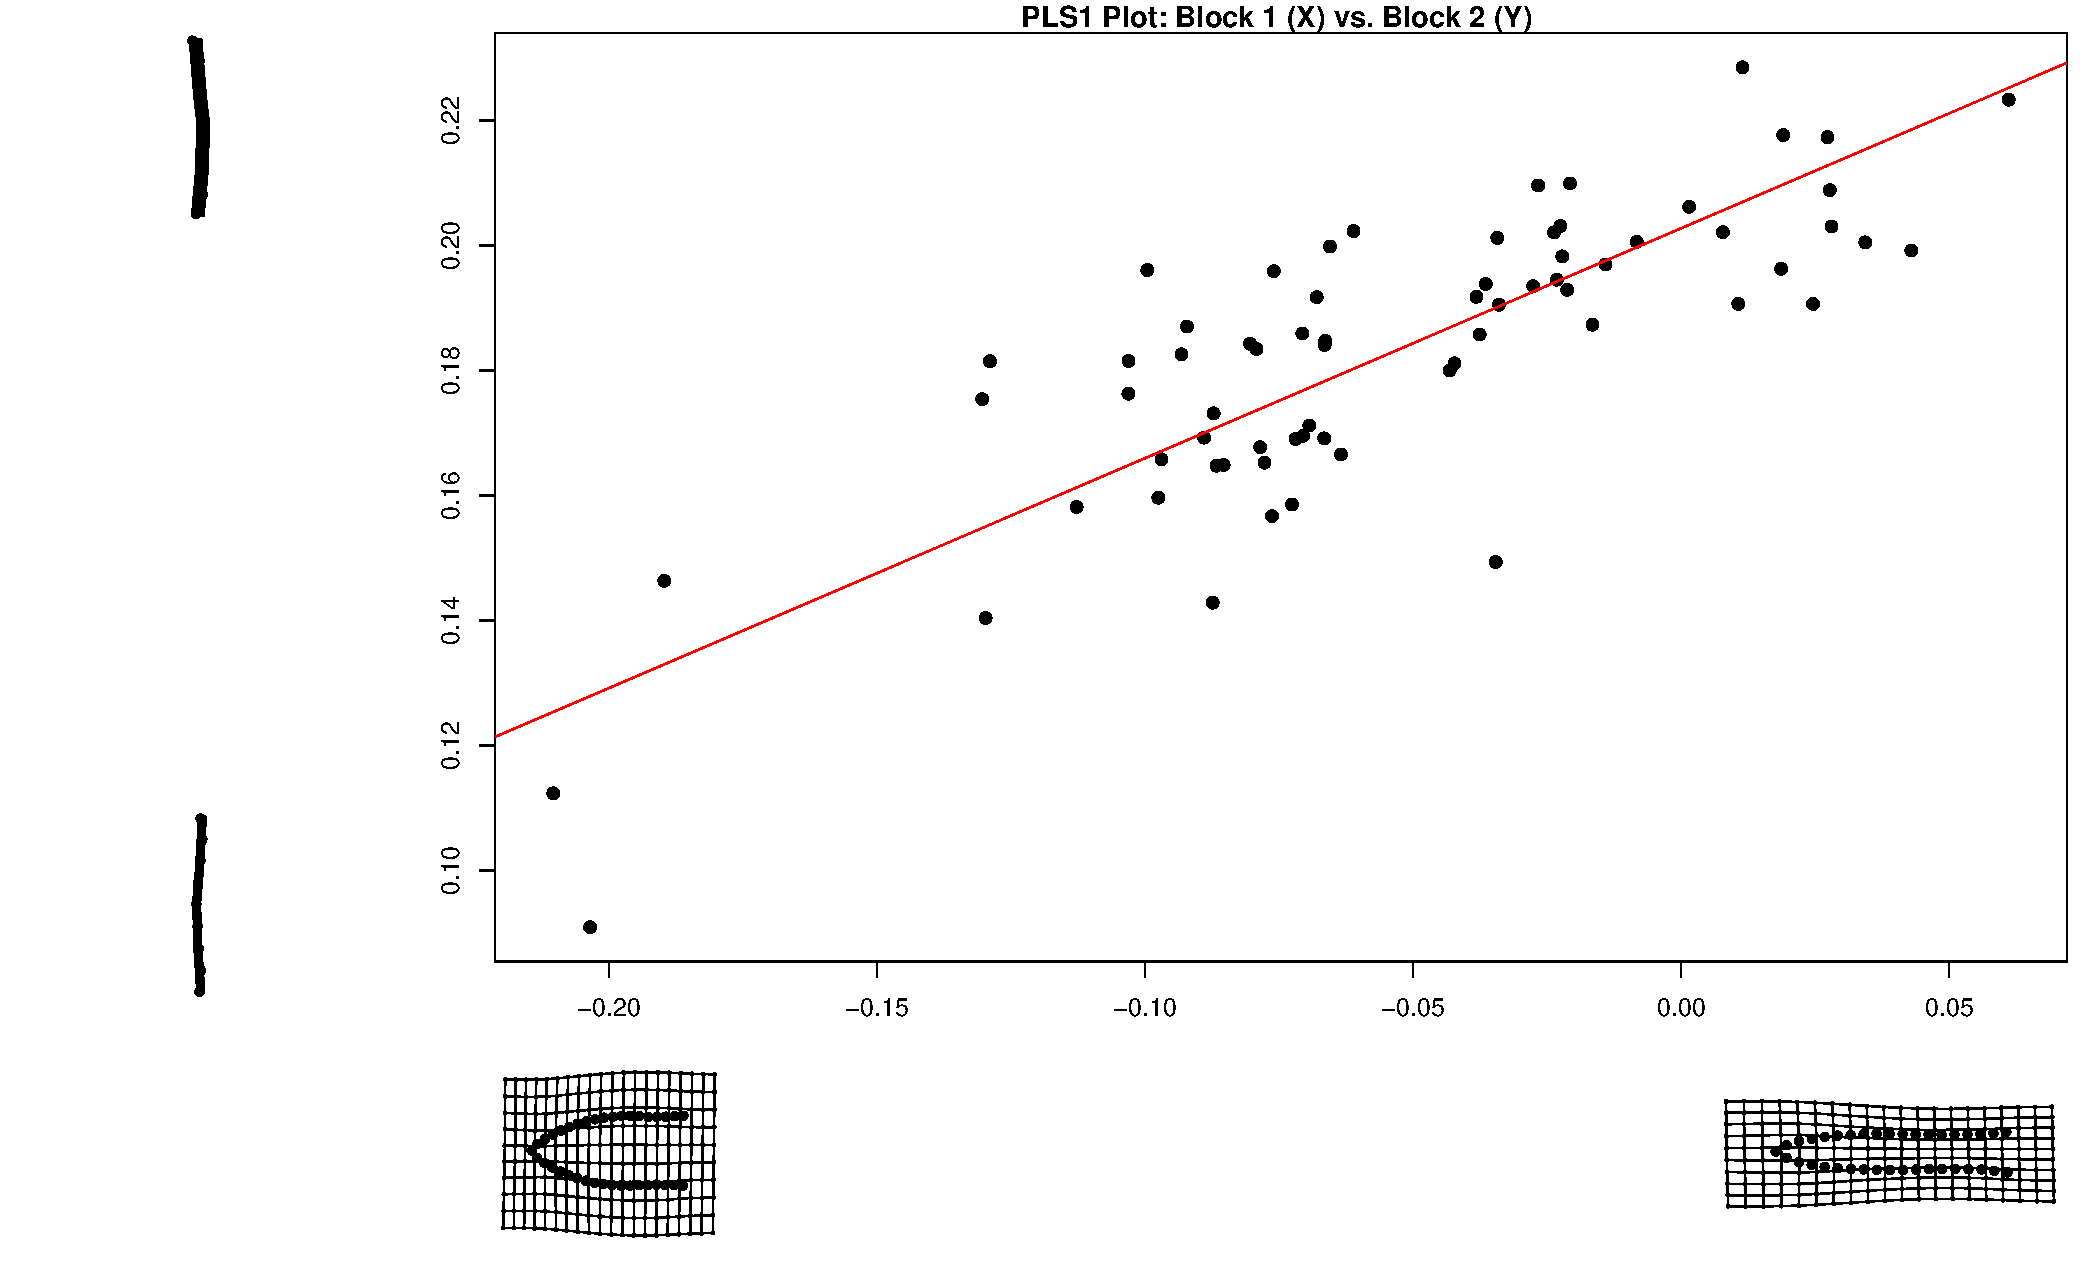
\includegraphics[width=\linewidth]{gahagan-morphinteg}
\caption{Two-block partial least-squares analysis for morphological integration of blade and base shape with singular warps illustrated.}
\label{fig:FigMorphInteg}
\end{figure}

A comparison of mean consensus configurations was used to further characterise the intra-site shape variation of Gahagan bifaces from Mounds Plantation, Gahagan Mound, and George C. Davis (Figure ~\ref{fig:FigMeanShp}). While those comparisons visualised in Figure ~\ref{fig:FigMeanShp}a and b were found to represent significant differences in biface morphology, the comparison in Figure ~\ref{fig:FigMeanShp}c was not. The subsequent test of directional asymmetry yielded results that were not significant.

\begin{figure}[ht]\centering
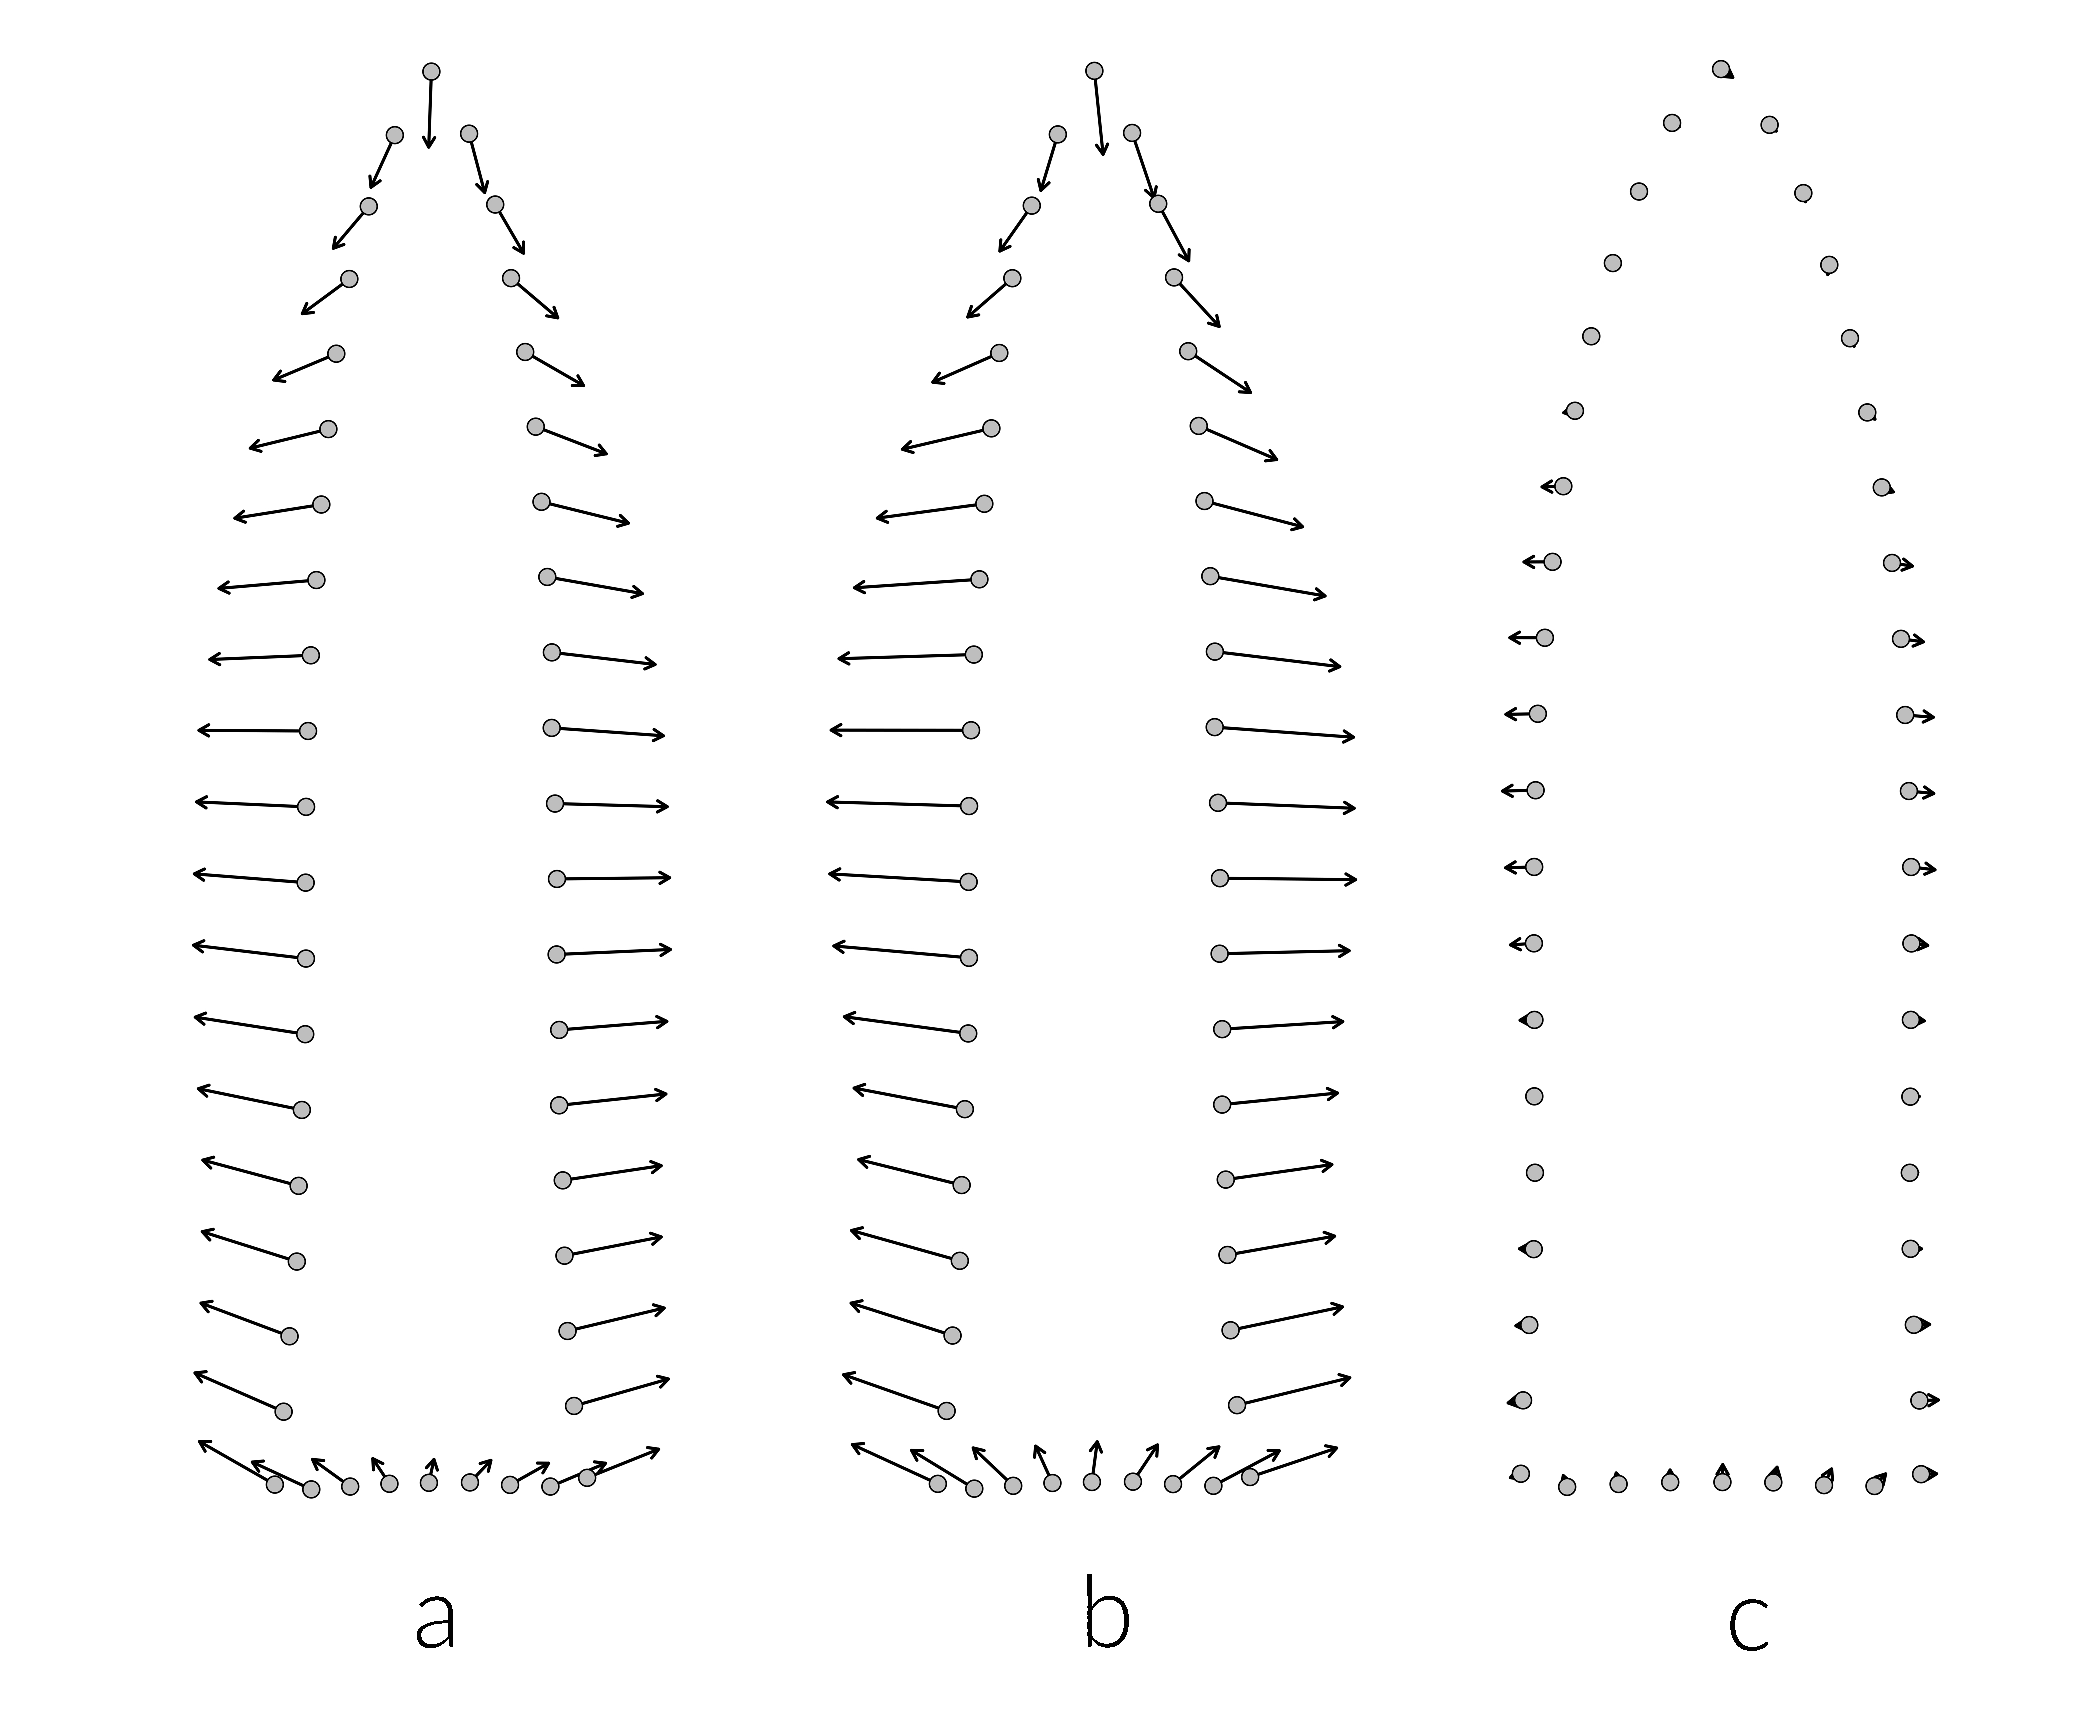
\includegraphics[width=\linewidth]{ref-to-target}
\caption{Comparison of mean consensus configurations for Gahagan biface shape by site at; a, Mounds Plantation (gray) and Gahagan Mound; b, Mounds Plantation (gray) and George C. Davis; c, Gahagan Mound (gray) and George C. Davis.}
\label{fig:FigMeanShp}
\end{figure}

\section{Discussion}

This comparison of the three largest assemblages of Gahagan bifaces from the Southern Caddo Area demonstrates a significant difference in the shape of bifaces produced at Mounds Plantation when compared with Gahagan Mound and George C. Davis. The test of morphological disparity revealed that Gahagan bifaces from the Gahagan Mound site include a significantly greater range of shapes than the Mounds Plantation sample, and the test of morphological integration indicated that the base and blade shapes of Gahagan bifaces vary in a coordinated manner. Lastly, the comparison of mean consensus configurations highlights that Gahagan bifaces from the Gahagan Mound site generally exhibit a lower degree of blade recurvature and a less convex base than those from the George C. Davis site.

\begin{figure}[ht]\centering
\includegraphics[width=\linewidth]{GMD}
\caption{Illustrated sample of Gahagan bifaces from the Gahagan Mound site demonstrating the morphological variation that occurs in Gahagan biface shape at the type site.}
\label{fig:GMD}
\end{figure}

If it is assumed that Gahagan bifaces were produced at or near their location of recovery (an assertion that may differ for the George C. Davis assemblage \citep{RN3682}), then results demonstrate that those bifaces produced at Mounds Plantation differ significantly in shape from the other assemblages (Table ~\ref{tab:Tbl3x} and Figure ~\ref{fig:FigPCA}), and occupy a more restricted range of morphospace than those produced at the type site (Table ~\ref{tab:Tbl4x} and Figure ~\ref{fig:FigMeanShp}). Results imply spatial production differences in northern (above the confluence of Cypress Bayou and the Red River) and southern (below) Caddo sites that align with recent findings associated with Hickory Engraved and Smithport Plain Caddo bottles from the same area \citep{RN11801,RN11716}, and also demonstrate that Caddo makers at the Mounds Plantation site were enlisting a more standardised approach to the manufacture of Gahagan bifaces (Table ~\ref{tab:Tbl4x}). This would similarly imply that Caddo makers at the Gahagan Mound site were producing Gahagan bifaces with a significantly greater range of morphological diversity (Table ~\ref{tab:Tbl4x} and Figure ~\ref{fig:GMD}). However variable, the morphology of Gahagan bifaces is not without pattern, as blade and base shapes can be said to covary throughout the sample (Figure ~\ref{fig:FigMorphInteg}). While additional research is warranted, this result implies that retouch of Gahagan bifaces was not arbitrary; rather, it was a practice constrained to a suite of blade and base shapes that vary in a coordinated manner.

"Standardization refers to homogeneity in ... materials, ... shape, and/or decoration" \citep[622]{RN28}, while diversity "can be most generally considered as the opposite of standardization" \citep[273]{RN18}. Standardisation is relative \citep{RN387,RN13}, and seen as a cultural marker that may have utility in a variety of interpretations. Attributes associated with standardisation may prove dynamic, potentially indicating periods of standardised production as well as periods of creativity that more readily articulate with diversity \citep{RN7}. In production contexts, standardisation might be seen as the result of minimised labour costs and improvements in efficiency \citep{RN13}. Both standardisation and diversity have utility in characterising tolerance, where a greater range of shapes may be indicative of a higher tolerance, and where lower tolerances can be demonstrated by production where variation is decreased \citep{RN35}. In this application, those bifaces from the Mounds Plantation site potentially represent production under a model of lower tolerance than those produced at the Gahagan Mound site, where the tolerance to morphological diversity appears higher.

Production activities are more likely to be localised than exchange systems, and are assumed to leave a clearer signature \citep{RN29}; in this case, those variables used in the analysis are the products themselves. The morphological attributes are representative of \textit{intentional attributes} \citep{RN250} related to morphological characteristics; in this instance, the blade and base of Gahagan bifaces. Dimensional standardisation has utility in identifying the range of variation and the overlap of product morphology within and between communities \citep{RN5897}. In this study, the relative dimensional standardisation exhibited at the Mounds Plantation site may imply a smaller number of production units (sensu \citet{RN29}) contrasted with a larger number of production units at the Gahagan Mound site. 

\section{Conclusion}

Through the use of morphological attributes associated with the blade and base shapes of Gahagan bifaces, a significant difference in morphology was found to occur at the Mounds Plantation site, where the range of morphological variation is also significantly more restricted when compared with Gahagan bifaces from the Gahagan Mound site. These results point toward a lower threshold for morphological variability at the Mounds Plantation site, which may indicate a smaller number of production units. While additional research is warranted, these findings articulate with a shift in Hickory Engraved and Smithport Plain bottle morphology over the same (north-south) geography \citep{RN11801,RN11716}, potentially indicating two previously unrecognised and morphologically-distinct Caddo lithic and ceramic production areas. 

\section*{Acknowledgments}

We extend our gratitude to the Caddo Nation of Oklahoma, Northwestern State University (Williamson Museum), the Louisiana State Exhibit Museum, and the Texas Archeological Research Laboratory for the requisite permissions and access needed to generate the 3D scans of the Gahagan bifaces. Thanks also to Dean C. Adams, Emma Sherratt, Timothy K. Perttula, Jeffrey R. Girard, Hiram F. (Pete) Gregory, and Kersten Bergstrom for their constructive criticisms, comments, and suggestions throughout the development of this research design, and to the anonymous reviewers for their comments and constructive criticisms, which further improved this manuscript. Components of this analytical work flow were developed and funded by a grant (P14AP00138) to RZS from the National Center for Preservation Technology and Training.

\section*{References Cited}

\bibliography{mybibfile}

\end{document}